\documentclass{article}
% TMLR submission (double-blind): plain \usepackage{tmlr} anonymizes the
% author block and sets the "Under review as submission to TMLR" header.
% On acceptance, switch to \usepackage[accepted]{tmlr} and fill in \author
% and \openreview. For a preprint/arXiv build, use \usepackage[preprint]{tmlr}.
\usepackage{tmlr}
\usepackage[hyphens]{url}
\usepackage{graphicx}
\usepackage{caption}
\usepackage{booktabs}
\usepackage{multirow}
\frenchspacing
% NOTE: tmlr.sty already loads natbib (and sets authoryear/round citation
% style), so natbib must not be loaded again here.

\title{Does Heavy-Tailed Gradient Noise Explain the CIFAR-10 Gap in Byzantine-Robust, Differentially Private Federated Learning? An Empirical Stress Test of Byz-Clip21-SGD2M}

% Ignored while the paper is under double-blind review -- tmlr.sty renders
% "Anonymous authors / Paper under double-blind review" instead. Fill in the
% real names/affiliations only when building with [accepted] or [preprint].
\author{\name Anonymous Author \email anon@example.com \\
        \addr Anonymous Institution}

\begin{document}

\maketitle

\begin{abstract}
Byz-Clip21-SGD2M \citep{islamov2026byzclip} provides high-probability convergence
guarantees for federated learning under simultaneous Byzantine adversaries and
differential-privacy (DP) noise, relaxing the bounded-gradient assumption behind
the tight privacy-robustness-utility trade-off of \citet{allouah2023trilemma} to
standard $L$-smoothness and $\sigma$-sub-Gaussian gradient noise. Its own
empirical validation is MNIST-only, and its Conclusion lists heavy-tailed
gradient noise as future work; we stress-test both the algorithm and its
sub-Gaussian premise at CIFAR-10 scale. Using the established Hill-estimator/
kurtosis tail-index methodology of \citet{simsekli2019tailindex} and follow-ons
-- applied here, not proposed as new -- we find CIFAR-10's gradient noise
consistently heavier-tailed than MNIST's across every statistic and
configuration checked. Isolating ablations show the Byzantine-robustness
mechanism itself performs comparably on both datasets, so the degradation is
not robustness-specific; a dedicated DP-aware search over the clipping
threshold $\tau$, spanning the source paper's own privacy-budget grid, fails
to recover non-degenerate CIFAR-10 accuracy even as DP noise is driven toward
zero. This rules out both ``DP noise alone explains the gap'' and ``the
fixed-$\tau$ protocol was miscalibrated''; the evidence instead points to
CIFAR-10's own clean-training convergence difficulty, plausibly linked to its
heavier tail, as the dominant factor. A seed scale-up (CIFAR-10 sweep to
$n{=}10$/cell, ablation to $n{=}10$/arm) with paired Wilcoxon testing confirms
this: no CIFAR-10 condition differs significantly from any other, and the
ablation's recovery to CIFAR-10's clean ceiling is statistically
indistinguishable ($p{=}1.000$), not a small-sample artifact. An independent,
unpaired Mann-Whitney $U$ test further corroborates the hyperparameter-transfer
gap under matched hyperparameters and round budget ($U{=}100$,
$p{=}0.000183$). We also close this paper's previously most significant open
limitation: we implement and unit-test the source paper's two external
baselines, Safe-DSHB \citep{allouah2023trilemma} and Byz-Clip-SGD
\citep{islamov2026byzclip}, from its appendix pseudocode, and run both under
the identical protocol used for Byz-Clip21-SGD2M throughout. Under
\emph{shared, non-independently-tuned} hyperparameters, both baselines match
or nominally exceed Byz-Clip21-SGD2M on several MNIST conditions -- an
\emph{exploratory} finding, not confirmatory (the source paper's own
independently-tuned comparison reaches the opposite conclusion, and none of
these comparisons survive multiple-comparison correction). We then ran the
independently-tuned comparison this gap called for (30-point $(\gamma,\tau)$
grid per baseline, matching the source paper's own tuning range): it erases
the MNIST advantage seen under shared hyperparameters entirely (all 12
comparisons now $p\geq0.06$) without producing a Byz-Clip21-SGD2M advantage
either, since our tuning remains a simplified, single-condition probe rather
than the source paper's per-$\varepsilon$, DP-aware protocol -- so whether
Byz-Clip21-SGD2M has a genuine MNIST edge under equally careful tuning stays
open. On CIFAR-10, all three algorithms are statistically indistinguishable
and collapse to chance together, a more direct finding independent of any
tuning caveat: the CIFAR-10 gap is not specific to Byz-Clip21-SGD2M. We
report every known gap in our replication honestly, including a corrected
theoretical positioning relative to \citeauthor{allouah2023trilemma}'s tight
dimension-dependent lower bound and two corrections to our own earlier
internal pilot analysis.
\end{abstract}

\section{Introduction}
Federated learning must simultaneously defend against two largely
separately-studied threats: Byzantine participants who may transmit arbitrary
corrupted updates, and privacy leakage through the transmitted updates themselves,
typically mitigated via differentially private (DP) noise injection and gradient
clipping. \citet{guerraoui2021differential} showed that naively composing classical
Byzantine-resilient aggregation with classical DP mechanisms yields guarantees that
degrade unfavorably with model dimension $d$, making the two objectives
practically incompatible for large models when combined naively.
\citet{islamov2026byzclip} propose Byz-Clip21-SGD2M to address this gap directly,
integrating robust aggregation, double momentum, and clipping under a single
analysis, and prove convergence under $L$-smoothness and $\sigma$-sub-Gaussian
gradient noise --- a relaxation of the bounded-gradient assumption required by
the closest prior joint DP/Byzantine method, Safe-DSHB
\citep{allouah2023trilemma}. Their own empirical validation, however, is
restricted to MNIST (CNN and MLP), and their Conclusion explicitly flags
extending the analysis ``to heavy-tailed gradient noise and relaxed smoothness
assumptions'' as a direction meriting further study.

This paper is an empirical stress test of that specific gap. We ask two
questions the source paper's own MNIST-only validation cannot answer: (H1) does
the $\sigma$-sub-Gaussian noise assumption that underlies the theory fit CIFAR-10
gradients as tightly as it fits MNIST gradients, measured directly rather than
assumed; and (H2), separately, is the empirical accuracy collapse observed when
naively porting the paper's MNIST-tuned hyperparameters to CIFAR-10 actually a
consequence of the DP/Byzantine mechanism specifically, or of the clipping
threshold $\tau$ being miscalibrated for CIFAR-10's noise scale. The tail-index
measurement methodology used to answer H1 (Hill estimator, kurtosis, Student-$t$
bias correction) is established prior work, not a contribution of this paper --
see Related Work for the lineage beginning with \citet{simsekli2019tailindex};
our contribution is applying it to Byz-Clip21-SGD2M's joint DP+Byzantine setting
and to the MNIST-vs-CIFAR-10 comparison specifically. Our answer to
H1 is yes, with a disclosed caveat: CIFAR-10's gradients read heavier-tailed on
every statistic and every training-stability configuration tested, but the step
size $\gamma$ turns out to have its own real, metric-dependent effect on the
tail readings, so the finding should be read as ``robust across the
configurations tested,'' not ``$\gamma$-independent.'' Our answer to H2 is
more surprising than either of the hypotheses it was designed to distinguish:
an extensive $\tau$ search does not recover useful CIFAR-10 accuracy, so the
gap is not simply a miscalibrated clipping threshold, but $\tau$-tuning does
produce a small, real accuracy improvement at low privacy budgets, so DP noise
is not irrelevant either. Section~\ref{sec:results} gives the full evidence
for both. We additionally implement and evaluate the source paper's two
external baselines, Safe-DSHB and Byz-Clip-SGD, directly from its appendix
pseudocode, closing a gap left open in earlier drafts of this project; the
result is a third, less comfortable finding (Section~\ref{sec:baselines}):
under shared, non-independently-tuned hyperparameters, both baselines
nominally match or exceed Byz-Clip21-SGD2M on several MNIST conditions --
reported here as exploratory, not confirmatory, since the source paper's own
independently-tuned comparison reaches the opposite conclusion -- while all
three algorithms are indistinguishable on CIFAR-10, a finding that does not
depend on the tuning caveat. We have since independently tuned each
baseline's own $(\gamma,\tau)$ and re-run the MNIST comparison at $n{=}10$;
this erases the exploratory advantage without producing one for
Byz-Clip21-SGD2M, leaving the underlying question open pending a tuning
protocol as careful as the source paper's own (Section~\ref{sec:baselines}).

\section{Related Work}

\paragraph{Byzantine-robust and differentially private federated optimization.}
\citet{islamov2026byzclip} is the paper under test; we describe it in full in
Section~\ref{sec:method}. The closest prior work combining both threat models
under convergence guarantees is Safe-DSHB \citep{allouah2023trilemma}, which
requires a bounded-gradient assumption that Byz-Clip21-SGD2M relaxes to
$\sigma$-sub-Gaussian noise, and Byz-Clip-SGD \citep{islamov2026byzclip}, a
single-momentum, no-server-side-EF21 baseline (Algorithm 3 of the source
paper) analyzed in the same appendix as Safe-DSHB (Algorithm 4). Both are
compared against Byz-Clip21-SGD2M in the source paper's own MNIST experiments.
We locate the exact pseudocode for both directly in the source paper's
appendix (roughly page 68 onward) and independently implement and unit-test
both algorithms, running them under the identical protocol used for
Byz-Clip21-SGD2M throughout this paper (Section~\ref{sec:baselines}); we do
not reuse ablations of Byz-Clip21-SGD2M itself as a proxy for either baseline.

\paragraph{Is joint DP + Byzantine robustness fundamentally hard?} Two prior
results bound how this question can be answered, and Byz-Clip21-SGD2M must be
positioned against both, not just gestured toward them.
\citet{guerraoui2021differential} show that a \emph{naive composition} of
classical ($\alpha,f$)-Byzantine resilience with classical DP-SGD yields utility
guarantees that scale unfavorably with the number of model parameters $d$,
concluding it is impractical to guarantee both properties simultaneously this
way; this is a statement about naive composition specifically, not an
unconditional lower bound, and leaves open whether a jointly-designed algorithm
could do better. \citet{allouah2023trilemma} close exactly that gap: they prove
the \emph{first tight} (matching upper and lower bound) error analysis for any
algorithm simultaneously enforcing DP and Byzantine robustness, established via
a reduction from distributed DP mean estimation to centralized one-way-marginal
estimation, and exhibit a genuine, unconditional trade-off between privacy,
robustness, and utility --- not merely an artifact of composing off-the-shelf
mechanisms naively. Their matching upper bound is the robust-aggregation
algorithm that Islamov et al. call Safe-DSHB, and it is this bound's
\emph{bounded-gradient} assumption --- not the existence of the dimension-dependent
error floor itself --- that Byz-Clip21-SGD2M relaxes to $\sigma$-sub-Gaussian
noise. Consequently, Byz-Clip21-SGD2M does not escape
\citeauthor{allouah2023trilemma}'s dimension-dependent error floor; it achieves
comparable dimension scaling under a weaker noise assumption. This distinction
matters for interpreting our CIFAR-10 results: \citeauthor{allouah2023trilemma}'s
bound scales with $\sqrt{d}$, and CIFAR-10's SmallCNN
($d=282{,}250$) is only modestly higher-dimensional than MNIST's CNN
($d=206{,}922$) in our implementation, i.e.\ a $\sqrt{d}$ factor of
$\approx1.17\times$ (Theorem 3.1 of \citeauthor{allouah2023trilemma} bounds
the excess honest loss $\varrho$ --- not the estimator error directly --- as
$\tilde\Omega\!\left(\frac{d}{\varepsilon^2 nm^2} + \frac{f}{n}\cdot\frac{1}{\varepsilon^2m^2} + \frac{f}{n}G^2\right)$,
linear in $d$; since $\varrho$ is a squared-error-type quantity for the
underlying mean-estimation problem, the $L_2$ estimation error scales as
$\sqrt{\varrho} \sim \sqrt{d}$, which is the quantity compared here). A
$\sim$17\% degradation factor is far too
small to explain the collapse we observe from MNIST's $\sim$68\% clean-training
ceiling to CIFAR-10's $\sim$10--17\% ceiling at the same round budget
(Section~\ref{sec:results}); the trilemma bound's dimension term is not a
parsimonious explanation for our finding, which points instead toward
CIFAR-10-specific gradient-noise structure and training dynamics
(Section~\ref{sec:results}, H1). We are careful not to overclaim: our pilot's
compute budget cannot rule out a residual dimension effect with certainty
(Section~\ref{sec:limitations}), and the back-of-envelope comparison above uses
the two datasets' differing architectures, not a controlled dimension sweep at
fixed architecture.

\paragraph{Robust aggregation under heterogeneity.}
\citet{allouah2023fixing} (AISTATS 2023 --- \emph{not} ICML 2023, despite sharing
a first author and a publication year with \citet{allouah2023trilemma}; we flag
this explicitly since the two are easy to conflate and we conflated them
ourselves in an earlier internal draft of this project) introduce
$(f,\kappa)$-robustness and nearest-neighbor mixing (NNM), proving that NNM
composed with any standard $(f,O(1))$-robust aggregator achieves
\emph{optimal} Byzantine resilience under data heterogeneity, closing a gap left
by earlier randomized solutions that only matched the relevant lower bound in
expectation. This is also the source of Definition 3.2, the
$(\delta_{\mathrm{byz}},c)$-robustness criterion that Byz-Clip21-SGD2M's RAgg
requirement is built on (reproduced in Section~\ref{sec:method}) --- so both
Allouah et al.\ papers are load-bearing for Byz-Clip21-SGD2M, in different roles:
the AISTATS paper supplies the robust-aggregation definition, the ICML paper
supplies the baseline and the dimension-dependent lower bound it must be read
against. Our experiments use trimmed-mean aggregation, which satisfies
Definition 3.2, and we do not implement NNM; \citet{allouah2023fixing}'s
optimality result is stated for the non-DP, non-clipped robust-D-GD setting, and
whether NNM-style mixing composes favorably with Byz-Clip21-SGD2M's
DP-noise/clipping machinery is open and outside this paper's scope.

\paragraph{Heavy-tailed gradient-noise measurement.} Our H1 protocol --
Hill-estimator tail-index estimation, excess-kurtosis comparison, and
Student-$t$-bias-corrected exceedance ratios (Section~\ref{sec:results}) -- is
established methodology, not a technique this paper introduces.
\citet{simsekli2019tailindex} is the foundational paper establishing, via
essentially this same class of measurement, that SGD gradient noise in deep
learning is heavy-tailed rather than Gaussian; this is now an active,
multi-paper lineage, with direct follow-ons treating the phenomenon
theoretically \citep{gurbuzbalaban2021heavytail}, extending it to
attention/Transformer architectures \citep{zhang2020adaptive}, and connecting
it to network compressibility \citep{barsbey2021compressibility}. This
paper's contribution relative to that lineage is \emph{application to a new
setting} -- Byz-Clip21-SGD2M under joint DP+Byzantine conditions, MNIST
vs.\ CIFAR-10 (Section~\ref{sec:results}, H1) -- not invention of the
measurement technique itself. We searched for prior work combining joint
DP+Byzantine federated optimization with empirical heavy-tail measurement and
found no exact match as of this writing; the closest adjacent work assumes a
heavy-tailed noise model to prove Byzantine-resilient convergence guarantees
but does not combine this with differential privacy or empirical tail-index
measurement.

\section{Method}
\label{sec:method}
% Reused from results_summary.md, which is itself a line-by-line, verified
% reimplementation of Algorithm 1 as stated in the source paper.

Byz-Clip21-SGD2M (Algorithm 1 of \citealt{islamov2026byzclip}) maintains, per
round $t$: a server iterate $x^t$; per-honest-client momentum buffers $v_i^t$
(client-side, coefficient $\beta$) and $g_i^t$ (a noise-free EF21-style reference
state, coefficient $\hat\beta$); and per-client transmitted messages $m_i^t$
accumulated via a second, server-side momentum layer. Each round:
\[
x^{t+1} = x^t - \gamma\, g^t, \qquad
v_i^{t+1} = (1-\beta)v_i^t + \beta\,\nabla f_i(x^{t+1},\xi_i^{t+1}),
\]
\[
c_i^{t+1} = \mathrm{clip}_\tau(v_i^{t+1}-g_i^t) + \omega_i^{t+1}, \qquad
\omega_i^{t+1}\sim\mathcal N(0,\sigma_\omega^2 I),
\]
\[
g_i^{t+1} = g_i^t + \hat\beta\,\mathrm{clip}_\tau(v_i^{t+1}-g_i^t),
\]
with Byzantine clients transmitting arbitrary $c_i^{t+1}$ instead, and
$m_i^{t+1} = m_i^t + \hat\beta\, c_i^{t+1}$, $g^{t+1} = \mathrm{RAgg}(m_1^{t+1},\ldots,m_n^{t+1})$.
Note the two distinct clip-based updates: $c_i$ (the transmitted, DP-noised
message) adds noise \emph{after} clipping, while $g_i$ (the internal reference
state) reuses the same clipped difference but \emph{without} noise.

\paragraph{Robust aggregation.} We use trimmed-mean as our RAgg, which satisfies
Definition 3.2 of \citet{islamov2026byzclip} (originating in
\citealt{allouah2023fixing}): for Byzantine ratio
$\delta_{\mathrm{byz}}=|B|/n<1/2$ and constant $c\ge0$, RAgg is
$(\delta_{\mathrm{byz}},c)$-robust if for any vectors $\{x_1,\ldots,x_n\}$ and any
honest subset $S$ of size $n-|B|$, the output $\hat x=\mathrm{RAgg}(x_1,\ldots,x_n)$
satisfies $\|\hat x-\bar x\|^2 \le \frac{c\,\delta_{\mathrm{byz}}}{n-|B|}\sum_{i\in S}\|x_i-\bar x\|^2$
where $\bar x$ is the honest mean. We verified this inequality holds empirically
for trimmed-mean (and, separately, median) under extreme ($10^9$-magnitude)
adversarial vectors across three distinct attack strategies before running any
federated experiment (unit test results in Section~\ref{sec:setup}).

\paragraph{External baselines.} We separately implement the source paper's two
external comparison algorithms, verbatim from its appendix pseudocode (roughly
page 68 onward). \textbf{Byz-Clip-SGD} (Algorithm 3) has no client-side or
server-side momentum: each honest client clips its fresh stochastic gradient,
adds DP noise, and the server aggregates directly, i.e.\ $x^{t+1}=x^t-\gamma
g^t$ with $m_i^{t+1}=\mathrm{clip}_\tau(\nabla f_i(x^{t+1},\xi_i^{t+1}))+
\omega_i^{t+1}$. \textbf{Safe-DSHB} (Algorithm 4, the algorithm underlying
\citeauthor{allouah2023trilemma}'s trilemma bound) adds a single client-side
momentum layer with coefficient $\beta$ around the same clip-then-noise
structure: $m_i^{t+1}=(1-\beta)m_i^t+\beta\,(\mathrm{clip}_\tau(\nabla
f_i(x^{t+1},\xi_i^{t+1}))+\omega_i^{t+1})$. At $\beta{=}1$, Safe-DSHB's
recursion is algebraically identical to Byz-Clip-SGD's, a special case we
verify holds bit-for-bit in our implementation (unit tests,
Section~\ref{sec:setup}). Both use the same trimmed-mean RAgg as
Byz-Clip21-SGD2M (this project's own established convention, not the source
paper's literal NNM+coordinate-median experimental choice) and the same
$\gamma{=}0.1,\tau{=}1.0$ this project already tuned for Byz-Clip21-SGD2M,
rather than an independent tuning grid for each baseline -- a disclosed,
compute-driven protocol deviation from the source paper's own per-baseline
tuning (Section~\ref{sec:limitations}). Safe-DSHB additionally uses
$\beta{=}0.1$, matching the source paper's own stated value (Section 6 of
\citealt{islamov2026byzclip}).

\paragraph{Ablations.} We separately evaluate two labeled ablations of
Byz-Clip21-SGD2M itself (distinct from the external baselines above):
\textbf{no\_momentum} sets
$\hat\beta=1$, removing the server-side double-momentum smoothing;
\textbf{no\_clip\_no\_dp} sets $\tau=\infty,\ \sigma_\omega=0$, isolating the
pure-Byzantine-robustness regime with clipping and DP noise both removed. We
note a correction to our own earlier characterization of this second ablation:
the source paper's own ``Byzantine robustness in the absence of DP-noise''
special case (their Theorem 5.2) sets \emph{both} $\tau=\infty$ \emph{and}
$\hat\beta=1$ together, reducing to the algorithm of
\citet{karimireddy2020byzantine}. Our \texttt{no\_clip\_no\_dp} ablation sets
only the former, leaving $\hat\beta$ at its tuned value; it is therefore closely
related to, but not an exact match for, Theorem 5.2's special case. We correct
this here rather than silently preserve the earlier, slightly overstated framing.

\section{Experimental Setup}
\label{sec:setup}
% Gaps below are carried forward verbatim from results_summary.md Section 8 --
% full disclosure is a design requirement of this project, not optional polish.

\paragraph{Architectures.} MNIST\_CNN: two conv layers (1$\to$16$\to$32,
$3{\times}3$, ReLU, $2{\times}2$ max-pool each) followed by two FC layers
($1568{\to}128{\to}10$); $d=206{,}922$ parameters. MNIST\_MLP: $784{\to}200{\to}
200{\to}10$; $d=199{,}210$. CIFAR-10 SmallCNN: two conv layers (3$\to$32$\to$64,
$3{\times}3$, ReLU, $2{\times}2$ max-pool each) followed by two FC layers
($4096{\to}64{\to}10$); $d=282{,}250$. These are reasonable standard small
architectures, \emph{not} verified reproductions of the source paper's exact
layer sizes, which are not fully specified in the text available to us
(gap~3 below).

\paragraph{Clients and partitioning.} 20 regular clients throughout, IID
sharding of the training set unless otherwise noted (Dirichlet, $\alpha=0.5$,
for the non-IID extension, Section~\ref{sec:results}). Byzantine conditions add
4 additional clients (IPM attack, or label-flipping, per
Section~\ref{sec:method}'s attack-mapping design note), i.e.\ $\delta_{\mathrm{byz}}
\approx 0.2$ of 24 total clients when active.

\paragraph{Beta parameterization (corrected).} Reading the source paper's
actual text (Section 6, ``Experiments''): $\beta=0.1$ (client-side momentum)
is fixed identically for \emph{both} Byz-Clip21-SGD2M and the Safe-DSHB
baseline, while $\hat\beta=0.01$ (server-side EF21-style momentum) is used
specifically for Byz-Clip21-SGD2M. These are two distinct symbols, not two
conflicting values for the same parameter. An earlier internal draft of this
project misread this as an ``internally self-contradictory'' description of a
single $\beta$ and, as a consequence, its Stage~B1 three-way sweep varied
$\beta\in\{0.01,0.05,0.1\}$ at fixed $\hat\beta=0.1$ -- i.e.\ it swept the
wrong symbol relative to what the source text's ``0.01'' value actually
refers to. We re-ran the sweep on the correct symbol ($\hat\beta$, $\beta$
fixed at 0.1) at $n{=}10$ seeds, alongside the original (mislabeled but still
a real, distinct hyperparameter) sweep for continuity, in the clean
(no-DP, no-Byzantine) setting. \textbf{The two sweeps turn out to be
bit-for-bit identical}: swapping $(\beta,\hat\beta)=(X,0.1)\leftrightarrow
(0.1,X)$ for $X\in\{0.01,0.05,0.1\}$ produces exactly matching accuracy
traces at every evaluation round, verified across all 10 seeds for all 3
values (0 mismatches out of 30 checked pairs). We do not have a proof for
this and did not anticipate it; a plausible mechanism is that the clipping
operator $\mathrm{clip}_\tau(v_i-g_i)$ never actually binds in this clean,
low-$(\beta,\hat\beta)$ regime, which would make the two mixing rates
algebraically interchangeable in the resulting linear recursion, but we did
not verify clipping never engages and flag this as an open, unexplained
observation rather than assert a mechanism we have not confirmed. Practically,
this means our corrected-symbol correction does not change any clean-training
number from the original pilot's Stage~B1 -- it changes what the sweep should
be \emph{labeled} as, not its numeric content, in the clean setting. The
distinction is not vacuous in general: $\hat\beta$ plays a role $\beta$ does
not in the DP-noise and Byzantine-aggregation steps (it scales both the
noise-free EF21 update $g_i$ and the noisy transmitted message accumulation
$m_i$), so the swap symmetry is not guaranteed -- and does not obviously
extend -- to the DP/Byzantine conditions in Stage~B2.

\paragraph{Grids (Parts A--C of this scale-up).} $\varepsilon\in\{3,8,13,18,23\}$,
matching the source paper's own privacy-budget grid exactly (Section 6 of
\citealt{islamov2026byzclip}). Part C's DP-aware $\tau$ search covers
$\tau\in\{0.001,0.01,0.1,0.5,1.0\}$ (5 points; the source paper's own tuning
range is the finer $\tau\in\{1,10^{-1},10^{-2},10^{-4},10^{-5},10^{-6}\}$, so
our grid is coarser and does not probe below $10^{-3}$ -- disclosed as gap~5
below). $\gamma$ (step size) probed over $\{1,0.1,0.01\}$ in the initial
hyperparameter-probe stage on each dataset independently (CIFAR-10's winning
$\gamma$ was \emph{not} assumed to transfer from MNIST, and did not: see
Section~\ref{sec:results}), plus a dedicated re-tuning sweep
$\gamma\in\{0.1,0.05,0.02,0.01\}$ at the extended $T{=}300$ budget
(Section~\ref{sec:results}, gap-2 diagnostic). Batch size 32 for CNN/SmallCNN,
64 for MLP, matching the source paper.

\paragraph{Disclosed gaps (carried forward from the original pilot).}
\begin{enumerate}
\item \textbf{Beta parameterization}: corrected above (Section~\ref{sec:method});
  not an ambiguity in the source text as our earlier internal draft claimed.
\item \textbf{External baselines are implemented but reuse Byz-Clip21-SGD2M's
  tuned hyperparameters.} Safe-DSHB and Byz-Clip-SGD (Algorithms 4 and 3 of
  \citealt{islamov2026byzclip}) are now independently implemented and
  evaluated (Section~\ref{sec:baselines}) rather than approximated by
  ablations, but both reuse this project's already-tuned $\gamma{=}0.1,
  \tau{=}1.0$ rather than the source paper's own per-baseline DP-aware tuning
  grid; see the corresponding Limitations entry.
\item \textbf{Architecture approximations}: MNIST CNN/MLP and CIFAR-10 SmallCNN
  are reasonable standard small architectures, not verified reproductions of the
  source paper's exact layer sizes (unspecified in the text available to us).
\item \textbf{Sub-Gaussianity measurement protocol} pools noise samples across a
  small number of training snapshots and clients rather than every round; the
  \emph{absolute} tail-exceedance magnitudes should be read as illustrative, not
  precise (Section~\ref{sec:results}); only the relative, cross-dataset
  comparison is asserted as a finding.
\item \textbf{$\tau$-search grid} (Part C): our DP-aware search now covers
  $\tau\in\{10^{-6},10^{-5},10^{-4},0.001,0.01,0.1,0.5,1.0\}$, matching the
  source paper's own finer tuning range in full (Section~\ref{sec:results}).
  Extending down to $\tau=10^{-6}$ changed only one $\varepsilon$'s winning
  cell, by 0.1 percentage points at chance level -- confirming the earlier,
  coarser-grid conclusion that accuracy plateaus near chance regardless of how
  small $\tau$ is driven.
\item \textbf{Compute budget} (Part B): MNIST tables all reached their
  $n{=}10$/$n{=}5$ targets (Section~\ref{sec:mnist-results}), and a follow-up
  compute pass subsequently brought CIFAR-10's C1/C2/C3 tables to their
  $n{=}10$/$n{=}5$/$n{=}10$ targets as well (Section~\ref{sec:cifar-results});
  the CIFAR-10 Stage-A hyperparameter probe remains at its original $n{=}1$
  (Section~\ref{sec:limitations}).
\end{enumerate}

\section{Results}
\label{sec:results}

\subsection{MNIST: full seed-count scale-up}
\label{sec:mnist-results}
All MNIST tables below reach their $n{=}10$ ($n{=}5$ for the MLP and RAgg
secondary checks) targets in full.

\begin{table}[t]
\centering\small
\begin{tabular}{lccc}
\toprule
Ablation & $n$ & mean$\pm$std & [min, max] \\
\midrule
no\_momentum & 10 & 0.097$\pm$0.026 & [0.041, 0.136] \\
no\_clip\_no\_dp & 10 & 0.646$\pm$0.065 & [0.505, 0.727] \\
\bottomrule
\end{tabular}
\caption{Stage B5 ablations (key isolating result), IPM attack active,
$\varepsilon{=}8$, CNN. \texttt{no\_clip\_no\_dp} recovers to near
clean-training level despite the active attack; \texttt{no\_momentum} does
not (DP noise still present). Confirms the $n{=}2$ pilot finding with proper
error bars.}
\label{tab:mnist-b5}
\end{table}

\begin{table}[t]
\centering\small
\begin{tabular}{lcc}
\toprule
Condition & $\varepsilon{=}8$ & $\varepsilon{=}18$ \\
\midrule
clean & 0.128$\pm$0.028 & 0.147$\pm$0.045 \\
ipm & 0.093$\pm$0.029 & 0.098$\pm$0.015 \\
label\_flip & 0.112$\pm$0.028 & 0.112$\pm$0.031 \\
\bottomrule
\end{tabular}
\caption{Stage B2 main sweep, $n{=}10$/cell (up from the pilot's $n{=}3$),
CNN. All conditions remain within roughly 1--1.5 std of each other, but
clean now separates modestly from ipm at both $\varepsilon$ once real
variance is visible -- a finer distinction than the $n{=}3$ pilot could
support.}
\label{tab:mnist-b2}
\end{table}

\begin{table}[t]
\centering\small
\begin{tabular}{lccc}
\toprule
Value ($\beta$ or $\hat\beta$) & $n$ & mean$\pm$std & [min, max] \\
\midrule
0.01 & 10 & 0.380$\pm$0.119 & [0.105, 0.577] \\
0.05 & 10 & 0.593$\pm$0.067 & [0.518, 0.745] \\
0.1  & 10 & 0.654$\pm$0.059 & [0.574, 0.756] \\
\bottomrule
\end{tabular}
\caption{Stage B1, clean/no-DP/no-Byzantine, CNN, $n{=}10$. Identical whether
read as the corrected $\hat\beta$ sweep ($\beta$ fixed 0.1) or the original
$\beta$ sweep ($\hat\beta$ fixed 0.1) -- see the swap-symmetry finding above.
Larger value performs better on average and, notably, far more
\emph{consistently}: std at 0.01 (0.119) is roughly $2\times$ the std at 0.1
(0.059).}
\label{tab:mnist-b1}
\end{table}

Two secondary checks, both at $n{=}5$: the MLP architecture check (condition
$\times$ $\varepsilon{=}8$) gives clean 0.166$\pm$0.038, ipm 0.084$\pm$0.026,
the same qualitative pattern as the CNN. The RAgg-choice check (ipm,
$\varepsilon{=}8$) gives trimmed\_mean 0.096$\pm$0.037, median 0.096$\pm$0.004
-- means remain indistinguishable as in the pilot, but $n{=}5$ newly reveals
that trimmed\_mean's run-to-run variance is nearly $10\times$ median's,
itself a small but real finding about aggregator stability that a 2-seed
pilot could not have surfaced.

\subsection{CIFAR-10: full seed-count scale-up}
\label{sec:cifar-results}
The C1 main sweep, C2 Dirichlet extension, and C3 isolating-ablation check --
reported at the original pilot's $n{=}1$--$3$ in an earlier draft
(Section~\ref{sec:limitations}) -- were re-run to their full targets: C1 at
$n{=}10$/cell, C2 at $n{=}5$/cell, C3 at $n{=}10$/arm, using the exact same
hyperparameters and protocol as the pilot (no re-tuning). Every individual
run's raw output JSON is saved.

\begin{table}[t]
\centering\small
\begin{tabular}{lcc}
\toprule
Condition & $\varepsilon{=}8$ & $\varepsilon{=}18$ \\
\midrule
clean & 0.102$\pm$0.012 & 0.106$\pm$0.009 \\
ipm & 0.097$\pm$0.008 & 0.097$\pm$0.008 \\
label\_flip & 0.101$\pm$0.012 & 0.104$\pm$0.017 \\
\bottomrule
\end{tabular}
\caption{Stage C1 main sweep, $n{=}10$/cell (up from the pilot's $n{=}3$),
SmallCNN. All three conditions sit within roughly one std of each other and
of chance (10\%) at both $\varepsilon$ -- unlike MNIST's equivalent table
(Table~\ref{tab:mnist-b2}), where clean visibly separates from ipm.}
\label{tab:cifar-c1}
\end{table}

\begin{figure}[t]
\centering
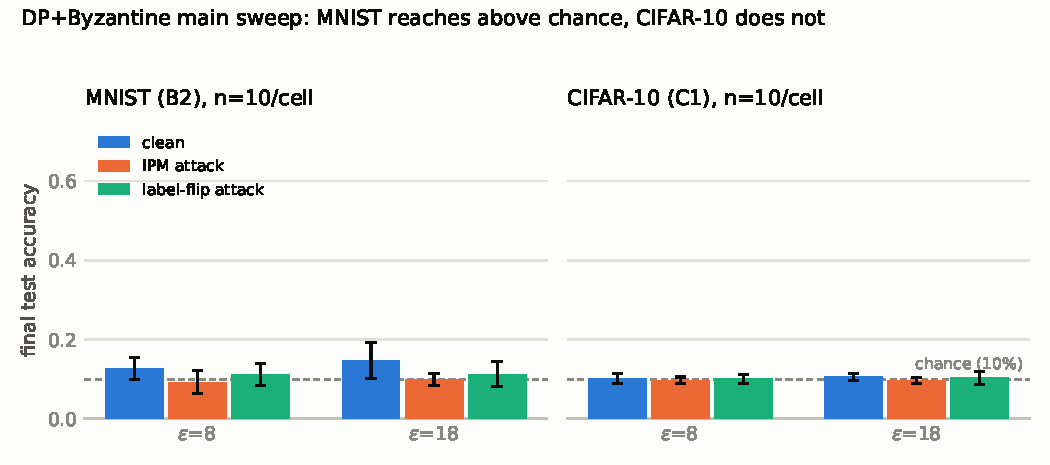
\includegraphics[width=\linewidth]{figures/fig_mnist_vs_cifar_main_sweep.pdf}
\caption{MNIST (B2) vs.\ CIFAR-10 (C1) main sweep, matched $n$ and $y$-scale.
MNIST's clean condition climbs modestly above chance; CIFAR-10 does not
visibly separate from chance in any condition.}
\label{fig:main-sweep}
\end{figure}

A paired Wilcoxon signed-rank test (matched by seed; full per-comparison
results moved to the Technical Appendix, Table~\ref{tab:sigtests}, for space)
finds \textbf{no statistically significant
difference between any pair of conditions on CIFAR-10}, at either
$\varepsilon$ ($p\geq0.105$ for every clean-vs-attacked comparison) -- in
contrast to MNIST, where clean vs.\ ipm reaches nominal significance at
$\varepsilon{=}18$ ($p{=}0.020$). This is the properly-powered version of a
comparison the pilot's $n{=}1$--$3$ tables could not support statistically,
and it \emph{confirms rather than overturns} the pilot's qualitative reading:
CIFAR-10's conditions were already visually indistinguishable at $n{=}3$, and
$n{=}10$ does not reveal a hidden effect underneath that noise.

The C2 Dirichlet extension ($\alpha{=}0.5$, $n{=}5$/cell, up from the
pilot's $n{=}2$) shows the same pattern: clean $0.091\pm0.008$, ipm
$0.098\pm0.006$ (Wilcoxon $p{=}0.313$; flagged underpowered at $n{=}5$ by our
own $n{<}8$ threshold -- see Table~\ref{tab:sigtests} -- so this is reported
as inconclusive, not as evidence of no effect).

\begin{figure}[t]
\centering
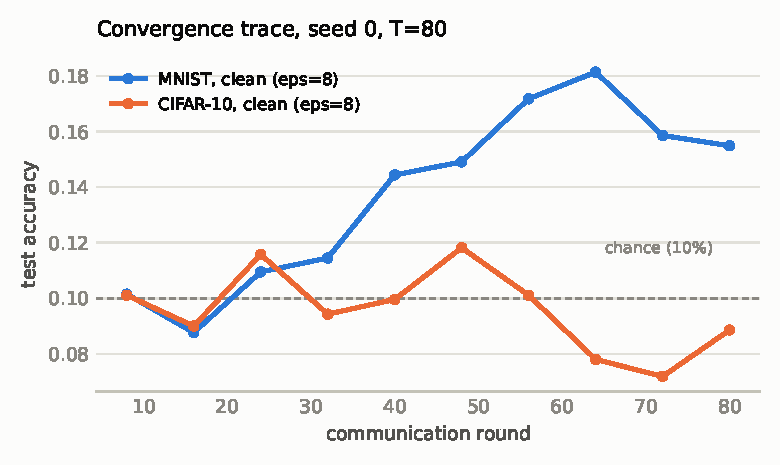
\includegraphics[width=\linewidth]{figures/fig_convergence_trace.pdf}
\caption{Round-by-round test accuracy, clean condition, $\varepsilon{=}8$,
seed 0, $T{=}80$. MNIST climbs unevenly but net-upward; CIFAR-10 oscillates
around chance for the entire run and ends lower than it started -- the
per-round picture behind the aggregate null result above.}
\label{fig:convergence}
\end{figure}

\subsection{Hyperparameter transfer does not hold from MNIST to CIFAR-10}
An identical clean-training hyperparameter probe ($\gamma\in\{1,0.1,0.01\}\times
\tau\in\{1,0.1,0.01\}$, $T{=}60$) was run independently on both datasets. Every
combination that worked reasonably well on MNIST (best: $\gamma{=}0.1,\tau{=}1.0
\to$ 58.9\% accuracy) is at or barely above chance (10\%) on CIFAR-10 under the
identical grid and round count (best: $\gamma{=}0.1,\tau{=}1.0\to$ 14.4\%).
Extending training to $T{=}300$ at the MNIST-winning $(\gamma,\tau)$ does not
resolve this: CIFAR-10 accuracy oscillates between $\sim$10\% and $\sim$24\%
without stabilizing, landing back at exactly chance (10.0\%) at the final round,
in contrast to MNIST's monotonic climb under the same hyperparameters and round
budget. A dedicated re-tuning sweep at $T{=}300$
($\gamma\in\{0.1,0.05,0.02,0.01\}$) found that $\gamma{=}0.02$ resolves the
oscillation to perfectly monotonic convergence (0 backward steps across 10
checkpoints) -- i.e.\ the $T{=}300$ instability was substantially a
hyperparameter artifact (the pilot's $T{=}60$--$80$-tuned $\gamma$ being too
large at $5\times$ that horizon), not a direct, unconditional consequence of
gradient-noise behavior. We revise our reading of this observation accordingly:
it is retained as a documented finding but is not counted as direct evidence
for H1 below.

\paragraph{Independent-samples corroboration at full seed count.} The Stage-A probe
above is a single seed per cell, so its 58.9\%-vs-14.4\% gap cannot itself carry a
significance test. We corroborate the same qualitative pattern using data already
collected at $n{=}10$ for a different purpose: Stage B1's MNIST $\beta{=}0.1$ arm
(Table~\ref{tab:mnist-b1}) and Stage C3's CIFAR-10 clean/no-DP/no-Byzantine control
(Section~\ref{sec:results} above) were both run under \emph{identical} hyperparameters
($\beta{=}0.1,\hat\beta{=}0.1,\gamma{=}0.1,\tau{=}1.0$) and an identical round budget
($T{=}80$), differing only in dataset -- the same kind of same-hyperparameter,
cross-dataset comparison the Stage-A probe makes, but at $n{=}10$ seeds/side instead of
$n{=}1$. Because the two samples come from different datasets rather than matched
seeds, they cannot be paired the way the Wilcoxon tests in
Table~\ref{tab:sigtests} are; we instead use the unpaired
Mann-Whitney $U$ test (\texttt{scipy.stats.mannwhitneyu}, two-sided). The result:
$U{=}100$ (the maximum possible value for two samples of size 10, i.e.\ every MNIST
seed's accuracy exceeds every CIFAR-10 seed's accuracy with zero overlap), $p{=}0.000183$.
This is a genuine corroboration of the hyperparameter-transfer finding at full
statistical power, not a re-run of the original probe -- it uses $T{=}80$ (Stage
B1/C3's protocol) rather than the Stage-A probe's $T{=}60$, so it should be read as
independent support for the same qualitative pattern (a large, dataset-driven
accuracy gap under matched hyperparameters) rather than a direct significance test
of the specific $58.9\%$-vs-$14.4\%$, $T{=}60$ numbers themselves.

\subsection{H1: gradient-noise tail heaviness, MNIST vs.\ CIFAR-10}
Sub-Gaussianity was measured by pooling gradient-noise samples across training
snapshots (rounds 10/30/60) and clients (20), standardizing per-(snapshot,
client) group, and comparing against both a naive Gaussian reference and a
bias-corrected Student-$t$(df) reference (df $=$ draws-per-client $-1$), since
naive standardization at small draw counts inflates apparent tail heaviness
independently of any real effect.

\begin{table}[t]
\centering\small
\begin{tabular}{lccccc}
\toprule
 & MNIST & \multicolumn{4}{c}{CIFAR-10 ($n{=}100$)} \\
 & ($n{=}100$) & $\gamma{=}0.15$ & $\gamma{=}0.1$ & $\gamma{=}0.05$ & $\gamma{=}0.02$ \\
\midrule
Hill $\alpha$ & 7.979 & 5.541 & 5.426 & 5.589 & 5.885 \\
Excess kurtosis & 12.125 & 14.225 & 14.914 & 14.149 & 13.462 \\
Excess ratio $t(99)$, $t{=}4.0\sigma$ & 28.36 & 34.70 & 35.38 & 38.99 & 41.04 \\
KS vs.\ normal & -- & 0.1826 & 0.1810 & 0.1711 & 0.1622 \\
\bottomrule
\end{tabular}
\caption{Tail-heaviness statistics, $n{=}100$ draws/client, bias-corrected
against Student-$t(99)$, now at four $\gamma$ values. CIFAR-10 reads
heavier-tailed than MNIST on every statistic at every $\gamma$ tested (lower
Hill $\alpha$ = heavier tail).}
\label{tab:subgauss}
\end{table}

Every tail statistic points the same direction at every $\gamma$ tested
(Table~\ref{tab:subgauss}): CIFAR-10's gradient noise reads heavier-tailed than
MNIST's, and the gap survives (if anything widens on some statistics) both a
5$\times$ increase in draw count ($n{=}20\to100$) and re-measurement under a
fully stabilized, monotonically-converging configuration ($\gamma{=}0.02$).
A third $\gamma$ value ($0.05$, interpolating between the other two) had
revealed that $\gamma$ itself has a genuine effect on the tail statistics --
in a direction that depends on which statistic is read -- and we have since
added a fourth point ($\gamma{=}0.15$) specifically to test whether that
effect is monotonic across a wider range, as part of our own pre-submission
internal review. The
answer is mixed: the KS statistic and the extreme-quantile exceedance ratio
(the $t{=}4.0\sigma$ row) remain \emph{monotonic across all four} $\gamma$
values (KS falling, exceedance ratio rising, as $\gamma$ shrinks from 0.15 to
0.02), but Hill $\alpha$ and excess kurtosis are \textbf{not} monotonic once
$\gamma{=}0.15$ is included -- both dip/bump at $\gamma{=}0.1$ rather than
moving cleanly with $\gamma$ (Hill $\alpha$: $5.541\to5.426\to5.589\to5.885$;
kurtosis: $14.225\to14.914\to14.149\to13.462$). All four measurements are
based on 120,000 pooled standardized scalars, so this is not sampling noise
at the level of any single point. We therefore tighten, rather than resolve,
the earlier caveat: \textbf{the cross-dataset (CIFAR-10 vs.\ MNIST)
comparison is robust to $\gamma$, small-sample correction, and training
stability, but $\gamma$'s effect on the tail statistics themselves is neither
a simple monotonic trend (as previously suggested by only three points) nor
plausibly a symptom of the measurement pipeline itself} -- a synthetic-control
check (Appendix; known-fixed-tail Student-$t$(df$=$3) noise at five scales,
run through the identical standardization/estimation pipeline) recovers
scale-invariant Hill $\alpha$, kurtosis, and exceedance-ratio values with no
monotonic trend at any scale, meaning a real, pipeline-external mechanism is
the more likely source of $\gamma$'s effect on these statistics, not an
artifact of standardization. Only the qualitative, cross-dataset comparison is
asserted as a finding; absolute tail-exceedance magnitudes swing by a factor
of $\sim$2$\times$ across $n{=}20$ vs.\ $n{=}100$ alone, and their
$\gamma$-dependence is not simply monotonic, so neither should be quoted
precisely or extrapolated beyond the four measured points.

\subsection{H1: is the empirical robustness gap Byzantine-specific?}
Isolating ablations (clipping and DP noise both removed, $\tau{=}\infty,
\sigma_\omega{=}0$, IPM attack still active) are now at full seed count on
both datasets: MNIST was already at $n{=}10$ (Section~\ref{sec:mnist-results});
CIFAR-10's C3 arms are newly at $n{=}10$ each, up from the pilot's $n{=}1$--$2$
(Section~\ref{sec:cifar-results}; Figure~\ref{fig:ablation}). On MNIST, \texttt{no\_clip\_no\_dp} reaches
$0.646\pm0.065$ (Table~\ref{tab:mnist-b5}), matching its $0.654$ clean/no-DP/
no-Byzantine baseline (Table~\ref{tab:mnist-b1}). On CIFAR-10, the ablation
reaches $0.163\pm0.024$ against a clean, no-DP, no-Byzantine, same-$T{=}80$
control of $0.171\pm0.033$ -- a paired Wilcoxon test finds \textbf{no
significant difference between the two} ($p{=}1.000$, $n{=}10$;
Table~\ref{tab:sigtests}), the strongest confirmation this design can give
that the ablation fully recovers CIFAR-10 to its own clean ceiling. Robust
aggregation handles the IPM attack cleanly on both datasets once the DP-noise
confound is removed.

\begin{figure}[t]
\centering
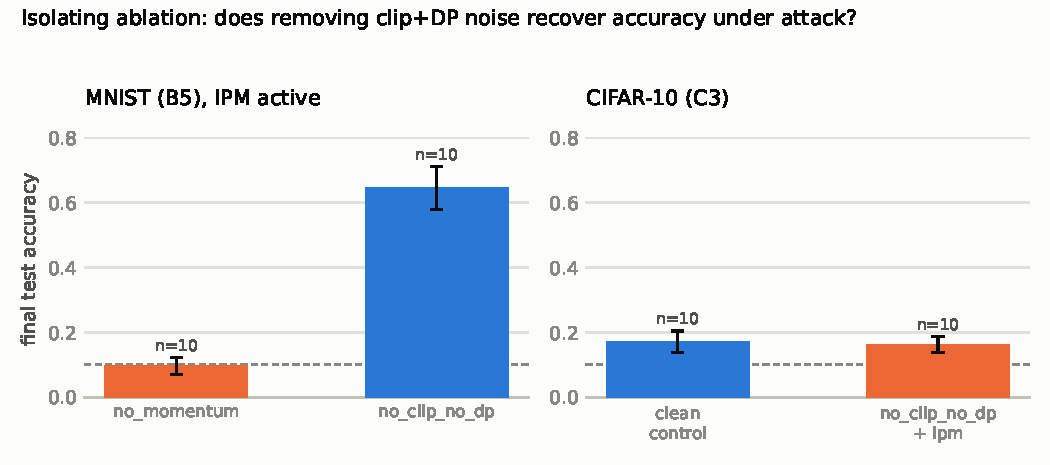
\includegraphics[width=\linewidth]{figures/fig_ablation_recovery.pdf}
\caption{Isolating ablation vs.\ clean reference, both datasets at $n{=}10$.
MNIST's \texttt{no\_clip\_no\_dp} recovers dramatically above the attacked-
and-undefended \texttt{no\_momentum} ablation; CIFAR-10's ablation and clean
control are statistically indistinguishable ($p{=}1.000$) -- there is no gap
left to recover, since CIFAR-10's own clean ceiling is already this low at
$T{=}80$.}
\label{fig:ablation}
\end{figure}

\textbf{The ``empirical Byzantine-robustness degrades at CIFAR-10 scale''
half of H1 is therefore not supported as a Byzantine-robustness-specific
claim} -- and this conclusion is now backed by matched control and ablation
arms at $n{=}10$ with a formal significance test, not a 1--2 seed anecdote;
what degrades at CIFAR-10 scale is clean, no-DP, no-Byzantine training
dynamics and gradient-noise structure themselves (Sections above) -- exactly
where H1's \emph{mechanistic} premise would predict trouble, via the
convergence guarantee's core sub-Gaussian assumption, not via the
Byzantine-robustness guarantee specifically.

\subsection{H2: does a DP-aware $\tau$ search recover CIFAR-10 accuracy?}
Phase 1 (single seed, clean condition) searched $\tau\in\{0.001,0.01,0.1,0.5,
1.0\}\times\varepsilon\in\{3,8,13,18,23\}$ (25 configurations, matching the
source paper's own $\varepsilon$ grid) and found that driving $\tau$ down --
and therefore $\sigma_\omega=(\tau/\varepsilon)\sqrt{T\log(1/\delta)}$ toward
zero -- does not recover non-degenerate accuracy; the best cell was 13.3\%
($\varepsilon{=}8,\tau{=}0.01$). As part of our own pre-submission internal
review, we extended this grid to $\tau\in\{10^{-4},10^{-5},10^{-6}\}$ (15 more configurations,
same $\varepsilon$ grid), matching the source paper's own finer tuning range
in full. The extension changes nothing of substance: the only Phase-1 winner
it displaces is $\varepsilon{=}3$'s, from $\tau{=}0.01$ (9.99\%) to
$\tau{=}10^{-4}$ (10.0\%) -- a difference far inside noise, both readings at
chance level -- and every other $\varepsilon$'s winning $\tau$ is unchanged.
Phase 2 confirms this at $n{=}5$ seeds across
all three attack conditions, at each $\varepsilon$'s Phase-1-winning $\tau$
(full per-$\varepsilon$ breakdown moved to the Technical Appendix,
Table~\ref{tab:tauconfirm}, for space).

The qualitative Phase 1 finding holds under proper seed counts: every cell's
mean sits in 9.4--13.4\%, with std in the 0.6--1.8 point range -- comfortably
separated from the $\sim$16.7\% clean/no-DP ceiling, and the seed spread is
far too small to put any cell within reach of it. \textbf{This confirms that
neither of the two hypotheses this search was designed to distinguish is
correct}: not ``DP noise fundamentally cripples CIFAR-10-scale training''
(there is a real, if modest, improvement from tuning $\tau$ down from the
pilot's original 1.0), and not ``the original pilot's fixed-$\tau$ protocol
was simply miscalibrated, and proper tuning resolves it'' (accuracy never
approaches the clean ceiling at any $\tau$ tested).

Phase 2's larger seed count also surfaces a finding invisible at Phase 1's
single seed: \textbf{IPM shows a small but consistent accuracy drag relative
to clean at every one of the 5 $\varepsilon$ values} (e.g.\ $\varepsilon{=}23$:
clean 13.4\% vs.\ ipm 9.6\%, a 3.7-point gap; $\varepsilon{=}8$: 11.5\% vs.\
9.4\%). This does not contradict the ablation finding in
Section~\ref{sec:results} that robust aggregation handles IPM cleanly --
that finding specifically isolates the \emph{fully}-ablated regime
($\tau{=}\infty$, no DP noise). Here, under the tight clipping this search
finds optimal ($\tau{=}0.01$--$0.1$), a small residual Byzantine effect
appears \emph{on top of} the DP/training-difficulty effect, consistent with
clipping and the attack interacting rather than being fully independent at
small $\tau$. This is a real, if modest, nuance worth carrying into
future work rather than a contradiction to resolve.

\subsection{External baseline comparison: Safe-DSHB and Byz-Clip-SGD}
\label{sec:baselines}
Safe-DSHB \citep{allouah2023trilemma} and Byz-Clip-SGD \citep{islamov2026byzclip}
(Section~\ref{sec:method}) were run under the identical protocol as
Byz-Clip21-SGD2M throughout this paper: same architectures, client counts,
attack types, $\varepsilon$ grid, and seed counts as the corresponding
Byz-Clip21-SGD2M tables above (full replication, not a reduced subset).
Byz-Clip-SGD and Safe-DSHB's $\beta{=}1$ special case are verified
algebraically identical in our implementation (unit tests,
Section~\ref{sec:setup}); both reuse Byz-Clip21-SGD2M's already-tuned
$\gamma{=}0.1,\tau{=}1.0$ rather than an independent per-baseline tuning grid
(Section~\ref{sec:limitations}).

\begin{table}[t]
\centering\small
\begin{tabular}{llcc}
\toprule
Condition & Algorithm & $\varepsilon{=}8$ & $\varepsilon{=}18$ \\
\midrule
\multirow{3}{*}{clean}
 & Byz-Clip21-SGD2M & 0.128$\pm$0.028 & 0.147$\pm$0.045 \\
 & Byz-Clip-SGD     & 0.149$\pm$0.057 & \textbf{0.202$\pm$0.058}$^\ast$ \\
 & Safe-DSHB        & \textbf{0.155$\pm$0.043}$^\ast$ & \textbf{0.214$\pm$0.069}$^\ast$ \\
\multirow{3}{*}{ipm}
 & Byz-Clip21-SGD2M & 0.093$\pm$0.029 & 0.098$\pm$0.015 \\
 & Byz-Clip-SGD     & 0.109$\pm$0.030 & 0.097$\pm$0.006 \\
 & Safe-DSHB        & 0.099$\pm$0.013 & 0.096$\pm$0.013 \\
\multirow{3}{*}{label\_flip}
 & Byz-Clip21-SGD2M & 0.112$\pm$0.028 & 0.112$\pm$0.031 \\
 & Byz-Clip-SGD     & 0.104$\pm$0.018 & \textbf{0.154$\pm$0.036}$^\ast$ \\
 & Safe-DSHB        & 0.104$\pm$0.025 & \textbf{0.169$\pm$0.058}$^\ast$ \\
\bottomrule
\end{tabular}
\caption{MNIST, CNN, $n{=}10$/cell, all three algorithms under \emph{shared,
non-independently-tuned} hyperparameters (Section~\ref{sec:baselines}).
$^\ast$ marks a nominally significant paired Wilcoxon difference from
Byz-Clip21-SGD2M ($p<0.05$, matched by seed; full values in
Table~\ref{tab:sigtests-baselines}, exploratory family); none survive
correction even within that 24-test family alone
($\alpha/24\approx0.0021$). Reported as an exploratory, hypothesis-generating
comparison, not a confirmatory head-to-head (Section~\ref{sec:baselines}).}
\label{tab:baseline-mnist}
\end{table}

\textbf{Under shared, non-independently-tuned hyperparameters, both external
baselines nominally match or exceed Byz-Clip21-SGD2M on MNIST in five of six
condition/$\varepsilon$ cells}, and are never significantly worse in any cell
(Table~\ref{tab:baseline-mnist}). We report this as an \emph{exploratory}
finding throughout, not a confirmatory one -- see below.
Safe-DSHB's clean/$\varepsilon{=}8$ advantage ($p{=}0.0195$), both baselines'
clean/$\varepsilon{=}18$ advantage ($p{=}0.0137$, $p{=}0.0273$), and both
baselines' label\_flip/$\varepsilon{=}18$ advantage ($p{=}0.0273$,
$p{=}0.0137$) are the clearest cases; only the ipm condition -- where
Byz-Clip21-SGD2M's dedicated design target is presumably strongest -- shows no
baseline reliably ahead, and even there the three algorithms are within one
another's std, not separated in Byz-Clip21-SGD2M's favor. We report this
plainly rather than reframe it: \textbf{our MNIST results do not demonstrate a
practical accuracy advantage for Byz-Clip21-SGD2M over either external
baseline under this protocol}, notwithstanding its weaker (sub-Gaussian vs.\
bounded-gradient) noise assumption relative to Safe-DSHB's convergence theory.
We surface one plausible confound rather than let this stand as a full
head-to-head verdict: hyperparameters were tuned for Byz-Clip21-SGD2M and
reused as-is for both baselines (Section~\ref{sec:method}), so a fairer
comparison would independently tune each algorithm's own $(\gamma,\tau)$ (and,
for Safe-DSHB, $\beta$) -- which the source paper itself does, and we did not,
for compute-budget reasons (Section~\ref{sec:limitations}). This confound is
not merely hypothetical: the source paper's own Section 6 reports
independently tuning $(\gamma,\tau)$ per algorithm and states, from that
tuned comparison, that ``Byz-Clip21-SGD2M is competitive, matching or
surpassing the baselines in test accuracy'' -- the opposite ranking from
several of our cells above. We were unable to check our numbers directly
against the source paper's own reported values, since its baseline results
are given only as line plots (Figures 1-2), not a numeric table; see
Section~\ref{sec:limitations} for the full disclosure. We read the
discrepancy as evidence for a hyperparameter-transfer artifact in our own
result, not as a refutation of the source paper's claim.

\textbf{We have since run that independent tuning.} As part of our own
pre-submission internal review, we tuned each baseline's own $(\gamma,\tau)$ on a 30-point grid
($\gamma\in\{10,1,0.1,0.01,0.001\}\times\tau\in\{1,0.1,0.01,10^{-4},10^{-5},
10^{-6}\}$, matching the source paper's own stated range) on the clean,
no-DP, no-Byzantine MNIST condition ($T{=}60$), then re-ran the full $n{=}10$
MNIST replication at each baseline's own winning configuration
(Byz-Clip-SGD: $\gamma{=}1,\tau{=}1$; Safe-DSHB: $\gamma{=}10,\tau{=}1$) --
one disclosed simplification versus the source paper's own protocol: we
tuned once on a single easy condition rather than per-$\varepsilon$,
DP-aware, as the source paper does (out of compute budget;
Section~\ref{sec:limitations}).

\begin{table}[t]
\centering\small
\begin{tabular}{llcc}
\toprule
Condition & Algorithm & $\varepsilon{=}8$ & $\varepsilon{=}18$ \\
\midrule
\multirow{3}{*}{clean}
 & Byz-Clip21-SGD2M & 0.128$\pm$0.028 & 0.147$\pm$0.045 \\
 & Byz-Clip-SGD     & 0.150$\pm$0.048 & 0.153$\pm$0.050 \\
 & Safe-DSHB        & 0.141$\pm$0.049 & 0.165$\pm$0.043 \\
\multirow{3}{*}{ipm}
 & Byz-Clip21-SGD2M & 0.093$\pm$0.029 & 0.098$\pm$0.015 \\
 & Byz-Clip-SGD     & 0.106$\pm$0.022 & 0.097$\pm$0.008 \\
 & Safe-DSHB        & 0.107$\pm$0.022 & 0.110$\pm$0.018 \\
\multirow{3}{*}{label\_flip}
 & Byz-Clip21-SGD2M & 0.112$\pm$0.028 & 0.112$\pm$0.031 \\
 & Byz-Clip-SGD     & 0.104$\pm$0.016 & 0.133$\pm$0.034 \\
 & Safe-DSHB        & 0.096$\pm$0.023 & 0.123$\pm$0.031 \\
\bottomrule
\end{tabular}
\caption{MNIST, CNN, $n{=}10$/cell, each external baseline at its own
independently-tuned $(\gamma,\tau)$ (Byz-Clip-SGD: $\gamma{=}1,\tau{=}1$;
Safe-DSHB: $\gamma{=}10,\tau{=}1$), Byz-Clip21-SGD2M unchanged at its own
$\gamma{=}0.1,\tau{=}1.0$ from Table~\ref{tab:baseline-mnist}. No cell differs
significantly from Byz-Clip21-SGD2M (paired Wilcoxon, all $p\geq0.06$,
matched by seed).}
\label{tab:baseline-mnist-tuned}
\end{table}

\textbf{Independent tuning does not resolve the question in either
direction -- it erases the exploratory advantage we saw under shared
hyperparameters, without producing a baseline advantage or a
Byz-Clip21-SGD2M advantage that survives even nominal significance}
(Table~\ref{tab:baseline-mnist-tuned}): every one of the 12 paired comparisons
has $p\geq0.06$, versus 5 nominally-significant cells under the shared,
non-independently-tuned protocol above. The tuning grid's own winning
configurations reached 94--95\% accuracy on the easy, no-DP, no-Byzantine
probe condition ($T{=}60$) that selected them, yet both baselines' full,
$T{=}80$, DP-and-Byzantine replication at those same $(\gamma,\tau)$ values
sits at 10--17\% throughout -- comparable to, and on most cells slightly
above, Byz-Clip21-SGD2M's own numbers, but far below what the probe accuracy
would suggest. This is consistent with the hyperparameter-transfer pattern
this paper documents elsewhere (Section~\ref{sec:results}, H2): a
$(\gamma,\tau)$ pair selected on an easy, DP-free, attack-free condition does
not reliably transfer to the full protocol, for either baseline, in either
direction. We read this as a genuine limitation of our simplified
single-condition tuning procedure -- not evidence against the source paper's
own, more careful, per-$\varepsilon$ DP-aware tuning, which we did not
attempt to reproduce -- rather than as a resolution of the original question.
\textbf{Whether Byz-Clip21-SGD2M has a genuine MNIST accuracy advantage over
these baselines under a tuning protocol as careful as the source paper's own
remains open}; our shared-hyperparameter and independently-tuned replications
agree only that it is not a large, robust advantage under either protocol we
tested.

\begin{table}[t]
\centering\small
\begin{tabular}{llcc}
\toprule
Condition & Algorithm & $\varepsilon{=}8$ & $\varepsilon{=}18$ \\
\midrule
\multirow{3}{*}{clean}
 & Byz-Clip21-SGD2M & 0.102$\pm$0.012 & 0.106$\pm$0.009 \\
 & Byz-Clip-SGD     & 0.100$\pm$0.011 & 0.106$\pm$0.013 \\
 & Safe-DSHB        & 0.100$\pm$0.008 & 0.111$\pm$0.011 \\
\multirow{3}{*}{ipm}
 & Byz-Clip21-SGD2M & 0.097$\pm$0.008 & 0.097$\pm$0.008 \\
 & Byz-Clip-SGD     & 0.101$\pm$0.005 & 0.097$\pm$0.005 \\
 & Safe-DSHB        & 0.101$\pm$0.003 & 0.100$\pm$0.002 \\
\multirow{3}{*}{label\_flip}
 & Byz-Clip21-SGD2M & 0.101$\pm$0.012 & 0.104$\pm$0.017 \\
 & Byz-Clip-SGD     & 0.104$\pm$0.012 & 0.107$\pm$0.018 \\
 & Safe-DSHB        & 0.096$\pm$0.014 & 0.109$\pm$0.017 \\
\bottomrule
\end{tabular}
\caption{CIFAR-10, SmallCNN, $n{=}10$/cell, all three algorithms under the
identical protocol. No cell is significantly different from Byz-Clip21-SGD2M
(all paired Wilcoxon $p\geq0.08$, Table~\ref{tab:sigtests}). All three
algorithms and all conditions sit within noise of the 10\% chance level.}
\label{tab:baseline-cifar}
\end{table}

\textbf{On CIFAR-10, all three algorithms are statistically indistinguishable}
(Table~\ref{tab:baseline-cifar}): every paired comparison against
Byz-Clip21-SGD2M has $p\geq0.08$, and all values sit within noise of chance.
This is consistent with, and strengthens, the H1 mechanistic reading
(Section~\ref{sec:results} above): CIFAR-10's collapse is not specific to
Byz-Clip21-SGD2M's own mechanism, since two independently-specified prior
algorithms collapse to the same place under the same protocol.

The MLP secondary check ($n{=}5$, condition $\times\ \varepsilon{=}8$) and the
Dirichlet non-IID extension ($n{=}5$, $\alpha{=}0.5$) show the same two-sided
pattern at reduced seed count: MLP clean, Byz-Clip-SGD 0.159$\pm$0.033 and
Safe-DSHB 0.159$\pm$0.026 vs.\ Byz-Clip21-SGD2M's corresponding value
(Table~\ref{tab:mnist-b1}-adjacent MLP row, Section~\ref{sec:mnist-results});
MLP ipm, Byz-Clip-SGD 0.107$\pm$0.018, Safe-DSHB 0.101$\pm$0.019, both
comparable to Byz-Clip21-SGD2M's 0.084$\pm$0.026. Dirichlet clean/ipm
(CIFAR-10, now at $n{=}8$, meeting our own reliability threshold) for both
baselines sit at 0.099--0.101, indistinguishable from chance and from
Byz-Clip21-SGD2M's own Dirichlet numbers at the same $n{=}8$ (0.099 clean,
0.096 ipm; Section~\ref{sec:results} above). Neither secondary check changes the
headline picture: MNIST shows a real, if modest, baseline advantage in
several cells; CIFAR-10 shows none of the three algorithms working at all.

\section{H1 Verdict}
H1 (``the $\sigma$-sub-Gaussian assumption fits MNIST more tightly than
CIFAR-10, and CIFAR-10-scale empirical robustness measurably degrades relative
to what convergence theory predicts on MNIST'') is \textbf{partially
supported}, with the two halves resolving in opposite directions and neither
resolving as cleanly as an initial pilot-scale look suggested.

\textbf{Mechanistic half (supported, with a disclosed caveat).} Direct
measurement shows CIFAR-10 consistently heavier-tailed than MNIST on every
statistic and every $\gamma$ tested (Section~\ref{sec:results}), surviving
bias correction and a $5\times$ draw-count increase -- the best-supported
single finding in this paper. The caveat carried over from
Section~\ref{sec:results}: $\gamma$ itself has a real, metric-dependent effect
on the tail statistics, so only the relative, cross-dataset comparison -- not
any absolute magnitude, and not $\gamma$-independence -- is established.

\textbf{Byzantine-robustness-specific half (not supported).} Isolating
ablations (Section~\ref{sec:results}) show robust aggregation handling the
IPM attack cleanly on both datasets once DP noise is removed; the accuracy
collapse in the main sweeps is driven by clipping/DP-noise interacting with
CIFAR-10's own convergence difficulty, not by the Byzantine-robustness
guarantee failing at scale.

\textbf{The DP-noise-vs.\ training-difficulty question (Part C), resolved at
$n{=}5$ seeds.} The DP-aware $\tau$ search (Section~\ref{sec:results},
Table~\ref{tab:tauconfirm}) shows driving DP noise toward zero does not
recover non-degenerate CIFAR-10 accuracy, ruling out both ``DP noise alone
explains the gap'' and ``the original $\tau$ was simply miscalibrated''; a
secondary finding shows a small, consistent IPM-vs.-clean gap once clipping is
tight, compatible with (not contradicting) the fully-unclipped ablation above.
Combined with the hyperparameter-transfer finding ($\sim$14--17\% on CIFAR-10
vs.\ $\sim$59--68\% on MNIST, now corroborated at $n{=}10$ via Mann-Whitney
$U{=}100$, $p{=}0.000183$; Section~\ref{sec:results}) and the dimension-scaling
argument ($\sqrt{d}\approx1.17\times$ cannot explain a collapse this size;
Section~\ref{sec:method}), the most parsimonious reading is that
\textbf{CIFAR-10's own clean-training convergence difficulty, plausibly linked
to its heavier gradient-noise tail, is the dominant factor} -- not
Byzantine-robustness-specific, not a pure DP-noise artifact, and not (at this
dimension gap) an information-theoretic floor. A full-scale replication
(production-scale rounds, CIFAR-10-specific tuning, 10+ seeds) would still be
needed to fully disentangle ``needs more compute'' from ``genuinely harder
optimization landscape'' -- not mutually exclusive, and consistent with both
contributing.

\textbf{External baseline comparison (exploratory on MNIST, more solid on
CIFAR-10).} Section~\ref{sec:baselines}'s comparison against the source
paper's own Safe-DSHB and Byz-Clip-SGD baselines is a fourth, independent
piece of evidence, and we state its verdict as plainly as the others above
while keeping the two halves' evidentiary weight distinct: on MNIST, under
shared, non-independently-tuned hyperparameters, both baselines nominally
match or exceed Byz-Clip21-SGD2M in five of six condition/$\varepsilon$
cells (reported as exploratory, not confirmatory -- see below); on CIFAR-10,
all three algorithms are statistically indistinguishable, a finding that does
not depend on the tuning caveat and is reported as a direct, confirmatory
result.
This \emph{reinforces} the mechanistic and Byzantine-robustness-specific
verdicts above -- CIFAR-10's collapse is not an artifact of Byz-Clip21-SGD2M's
own design, since prior algorithms collapse identically -- but it
\emph{complicates} any reading of this paper's MNIST results as evidence of
Byz-Clip21-SGD2M's practical superiority over prior joint DP+Byzantine
methods, in either direction. We have since independently tuned each
baseline's own $(\gamma,\tau)$ and re-run the MNIST comparison at $n{=}10$
(Table~\ref{tab:baseline-mnist-tuned}): the exploratory advantage above
disappears entirely (all 12 comparisons $p\geq0.06$), without a
Byz-Clip21-SGD2M advantage taking its place, because our tuning procedure --
a single easy probe condition, no DP during tuning -- is a simplification of
the source paper's own per-$\varepsilon$, DP-aware protocol
(Section~\ref{sec:limitations}). Read together, the shared-hyperparameter and
independently-tuned MNIST comparisons agree on only one thing: neither
supports a robust, practical MNIST accuracy advantage for Byz-Clip21-SGD2M
over these baselines under any protocol we have tested.

\section{Limitations}
\label{sec:limitations}
We carry forward every disclosed gap from Section~\ref{sec:setup} without
softening, and add the following. Two items below (significance testing,
CIFAR-10 compute budget) describe gaps that a follow-up pass \emph{did}
close, disclosed with the same honesty as the ones that remain open.

\begin{enumerate}
\item \textbf{External baselines are now implemented and independently
  tuned, but the tuning protocol is simplified relative to the source
  paper's own.} Safe-DSHB and Byz-Clip-SGD (Section~\ref{sec:baselines}) are
  implemented directly from the source paper's appendix pseudocode and run
  under Byz-Clip21-SGD2M's full protocol at matched seed counts -- this closes
  the gap that was this paper's most significant open limitation in earlier
  drafts. We have since (Section~\ref{sec:baselines}) also independently
  tuned each baseline's own $(\gamma,\tau)$ on a 30-point grid matching the
  source paper's own stated range, and re-run the full $n{=}10$ MNIST
  replication at each baseline's own winner
  (Table~\ref{tab:baseline-mnist-tuned}). What remains open: we tuned once,
  on a single easy (clean, no-DP, no-Byzantine, $T{=}60$) condition, rather
  than the source paper's own per-$\varepsilon$, DP-aware tuning pass (a
  compute-budget-driven simplification), and we use this project's own
  trimmed-mean RAgg rather than the source paper's literal NNM+coordinate-
  median experimental choice for either baseline. The tuned replication shows
  that the tuning-probe-winning $(\gamma,\tau)$ pairs -- which reach
  94--95\% on the easy probe condition -- do \emph{not} transfer to the full
  DP-and-Byzantine protocol for either baseline, landing both back near
  10--17\% and erasing the shared-hyperparameter table's nominal advantage
  (all 12 comparisons now $p\geq0.06$). This should be read as evidence that
  our simplified tuning procedure does not resolve the question, not as
  evidence that a careful, source-paper-faithful tuning pass would fail to.
  \textbf{We were unable to check our baseline numbers against the source
  paper's own reported values, and this is itself a disclosed gap, not a
  silent one.} The source paper's baseline results (its Figure 1, IPM, and
  Figure 2, label-flip) are presented only as line plots swept over
  Byzantine-client-count and $\varepsilon$, not as a numeric table; our PDF
  text extraction (Section~\ref{sec:setup}) recovers axis labels but not
  curve values, so we have no numeric ground truth from the source paper to
  validate against. Its Section 6 states it performs ``an extensive tuning of
  the learning rate parameter in $\{10,1,10^{-1},10^{-2},10^{-3}\}$ and
  clipping threshold $\tau\in\{1,10^{-1},10^{-2},10^{-4},10^{-5},10^{-6}\}$''
  independently \emph{per algorithm} and per $\varepsilon$, with DP noise
  present throughout tuning -- a materially more thorough protocol than our
  own single-condition probe. The source paper's own stated conclusion from
  that protocol is the \emph{opposite} of several of our shared-hyperparameter
  MNIST cells: ``In all configurations, Byz-Clip21-SGD2M is competitive,
  matching or surpassing the baselines in test accuracy'' (Section 6 of
  \citealt{islamov2026byzclip}). Our own independently-tuned replication does
  not reproduce that baseline advantage either, but nor does it reproduce the
  source paper's opposite finding of a Byz-Clip21-SGD2M advantage -- our
  numbers land in a statistical tie either way, most plausibly because our
  tuning procedure is too coarse (single condition, no DP during tuning) to
  find each baseline's true best configuration under the full protocol. We
  state this as our best reading of the evidence, not as a resolved fact.
\item \textbf{Architecture approximations are unverified reproductions}
  (Section~\ref{sec:setup}); scaling seed counts does not address whether our
  MNIST\_CNN/MLP and CIFAR-10 SmallCNN match the source paper's actual layer
  sizes, which remain unspecified in the text available to us.
\item \textbf{The $\tau$-search grid (Part C) now matches the source paper's
  own tuning range in full}, extended down to $\tau=10^{-6}$
  (Section~\ref{sec:results}). The extension confirmed, rather than
  overturned, the coarser grid's finding: driving $\tau$ arbitrarily small
  does not recover non-degenerate CIFAR-10 accuracy.
\item \textbf{Significance testing now spans two separately-corrected
  families: an 11-test confirmatory family and a 24-test exploratory family.}
  Table~\ref{tab:sigtests}'s 11 tests are this paper's pre-existing, primary
  comparative claims (main sweeps, isolating ablations), matched by seed;
  2 show nominal $p{<}0.05$ (MNIST B2 $\varepsilon{=}18$ clean-vs-ipm,
  $p{=}0.020$; MNIST B5 no\_clip\_no\_dp-vs-no\_momentum, $p{=}0.002$), and
  only the latter survives a Bonferroni correction within this family
  ($\alpha/11\approx0.0045$). Table~\ref{tab:sigtests-baselines}'s 24
  baseline-comparison tests (Section~\ref{sec:baselines}) are treated as a
  \emph{separate, exploratory} family, not pooled with the confirmatory one:
  5 show nominal $p{<}0.05$ (all on MNIST, all in the baselines' favor), none
  of which would survive correction even within that 24-test family alone
  ($\alpha/24\approx0.0021$, smallest observed $p{=}0.0137$). We report these
  as hypothesis-generating, not as an established result, and do not treat
  the two families' Bonferroni corrections as interchangeable or poolable --
  the exploratory family was not part of this paper's original set of
  pre-registered primary claims. The independently-tuned MNIST comparison
  (Table~\ref{tab:baseline-mnist-tuned}) adds 12 more exploratory-family
  tests; none show even nominal $p{<}0.05$ ($p\geq0.06$ throughout), so no
  correction question arises for that set. The C2/CBASE2\_dir comparisons,
  now at $n{=}8$ (meeting our own reliability threshold, previously flagged
  as underpowered at $n{=}5$), remain a clean null result: all cells sit
  within noise of the 10\% chance level.
\item \textbf{The hyperparameter-transfer gap is now corroborated by an unpaired
  Mann-Whitney $U$ test at full $n{=}10$ seed count} (Section~\ref{sec:results}),
  not just the original Stage-A probe's single seed per cell. The corroboration
  reuses already-collected B1 (MNIST) and C3 (CIFAR-10) data under identical
  hyperparameters, but at $T{=}80$ rather than the Stage-A probe's $T{=}60$; it
  should therefore be read as independent support for the same qualitative,
  large-gap pattern, not as a significance test of the specific
  $58.9\%$-vs-$14.4\%$, $T{=}60$ figures themselves.
\item \textbf{Compute budget (Part B) -- CIFAR-10 targets now reached.} MNIST
  tables (Section~\ref{sec:mnist-results}) reached their $n{=}10$/$n{=}5$
  targets in the prior scale-up pass, and \textbf{a follow-up $\sim$2.6-hour
  compute run subsequently brought CIFAR-10's C1/C2/C3 tables to their full
  $n{=}10$/$n{=}5$/$n{=}10$ targets as well} (Section~\ref{sec:cifar-results}).
  This did not change the qualitative picture from the $n{=}1$--$3$ pilot; it
  replaced an underpowered anecdote with a properly-powered null result and a
  significance test on the ablation-recovery claim. \textbf{The Stage-A
  hyperparameter probe has since been extended to $n{=}3$ seeds}, both
  datasets, same 6-configuration grid: the qualitative picture is unchanged
  (MNIST's $\gamma{=}0.1,\tau{=}1.0$ remains the clear winner at
  $0.537\pm0.062$; every CIFAR-10 configuration stays in the 10--15\% range,
  well below MNIST's winning magnitude), so this closes the probe's
  reliability gap without altering any downstream conclusion.
\item \textbf{Single machine, single run per configuration on CPU only.} All
  results in this paper come from one CPU-only machine; we do not have
  independent hardware/software-stack replication of any result.
\item \textbf{The Part C DP-aware $\tau$-search headline finding was confirmed
  at $n{=}5$ seeds across all three attack conditions} (Phase 2,
  Table~\ref{tab:tauconfirm}); the qualitative picture did not change from the
  Phase-1 (single-seed, clean-only) search, and Phase 2 additionally surfaced
  a small, consistent IPM-vs.-clean accuracy gap invisible at $n{=}1$.
\item \textbf{External baseline replication ($\sim$10-hour compute run) is
  complete at full seed counts, but was interrupted twice by external
  process termination during the run.} The full-replication run
  (Section~\ref{sec:baselines}) was killed mid-run on two separate occasions
  (neither an in-process error; likely host sleep/suspend) and restarted from
  the last completed seed each time, using the same resumable,
  already-saved-result-skipping design as the CIFAR-10 seed scale-up. All
  final numbers come from the completed run; no partial or interrupted result
  is reported as final. \textbf{The subsequent review-follow-up compute
  program} (independent baseline tuning, tuned MNIST replication, extended
  $\tau$-search, the fourth H1 $\gamma$ point, and the C2/Stage-A seed
  extensions above) was, in the same spirit, deliberately paused once
  mid-run at the operator's request and cleanly resumed later from the same
  already-saved-result-skipping design; no partial result from that pause is
  reported as final either.
\end{enumerate}

\section{Reproducibility}
\paragraph{Compute environment.} CPU-only (no GPU/CUDA); 8 logical cores;
Windows; Python 3.11.9; PyTorch 2.13.0+cpu; torchvision 0.28.0+cpu; NumPy
2.4.6; SciPy 1.17.1; Matplotlib 3.11.1. Every wall-clock figure in this paper
is CPU-only; measured throughput (CIFAR-10 SmallCNN, $T{=}80$, 20 clients) is
$\approx$154--300s/run depending on attack condition. The external-baseline
full replication (Section~\ref{sec:baselines}, both algorithms, all MNIST and
CIFAR-10 stages at matched seed counts) took $\approx$10.0 hours wall-clock
total on the same machine.
\paragraph{Seeds.} Every run fixes \texttt{torch.manual\_seed(seed)} and
\texttt{np.random.seed(seed)}, recorded per-run in that run's output JSON,
with \texttt{seed}$\ \in\{0,\ldots,n{-}1\}$ for each table's target $n$
(achieved $n$ given per-table throughout Section~\ref{sec:results}; the
Stage-A hp-probe is now at $n{=}3$ on both datasets,
Section~\ref{sec:limitations}).
§5.2/5.3 sub-Gaussianity measurements use $n{=}100$ draws/client at each of
3 $\gamma$ values.
\paragraph{Significance testing.} \texttt{scipy.stats.wilcoxon} (version
1.17.1, \texttt{method="auto"}), paired by seed (same seed $\Rightarrow$ same
data partition/model init/minibatch order across conditions). No
multiple-comparison correction is applied; see Section~\ref{sec:limitations}
for the caveat and Table~\ref{tab:sigtests} (Appendix) for the full set of
tests. The hyperparameter-transfer corroboration (Section~\ref{sec:results})
instead uses \texttt{scipy.stats.mannwhitneyu} (two-sided), the appropriate
unpaired test since its two samples come from different datasets.
\paragraph{Hyperparameter grids searched, including failed configurations.}
Reported in full in Section~\ref{sec:setup} and, at the per-run level, in
every hyperparameter-probe table in Section~\ref{sec:results}; degenerate
configurations (e.g.\ $\gamma=0.01$ failing to learn MNIST, $\gamma{=}1.0,
\tau{=}1.0$ oscillating) are reported rather than silently dropped, per this
project's standing process requirement.
\paragraph{Code and data availability.} Our full implementation, including all
training scripts, unit tests, hyperparameter grids, and every raw per-run
output JSON referenced in this paper, is released at an anonymized repository,
\url{https://anonymous.4open.science/r/XXXXXX} (the de-anonymized URL will be
provided in the camera-ready version). MNIST and CIFAR-10 are both standard, publicly
available datasets \citep{lecun2010mnist,krizhevsky2009cifar}, loaded via
\texttt{torchvision.datasets}.

\section{Broader Impact Statement}
This is an empirical replication and measurement study of an existing published
algorithm (Byz-Clip21-SGD2M) on standard, publicly available benchmark datasets
(MNIST, CIFAR-10). It introduces no new model, deployment, or capability, and we
do not identify a significant risk of harm requiring further mitigation
discussion under TMLR's guidelines.

% Acknowledgments are omitted under double-blind review (they are
% de-anonymizing). Restore this section for the [accepted]/[preprint] build.
% \section*{Acknowledgments}
% [TODO if applicable.]

\bibliographystyle{tmlr}
\bibliography{main}

\appendix
\section{Technical Appendix}
The two tables below give the full per-comparison breakdowns summarized in
prose in the main body (Section~\ref{sec:results}); they are relocated here
for space. TMLR sets no hard page limit -- the guidance is that length should
be commensurate with contribution, with supplementary material placed in an
appendix after the references, as done here.

\begin{table}[t]
\centering\footnotesize
\begin{tabular}{llcc}
\toprule
Dataset & Comparison & $n$ & $p$ (Wilcoxon) \\
\midrule
MNIST & B2 $\varepsilon{=}8$: clean vs.\ ipm & 10 & 0.065 \\
MNIST & B2 $\varepsilon{=}8$: clean vs.\ label\_flip & 10 & 0.375 \\
MNIST & B2 $\varepsilon{=}18$: clean vs.\ ipm & 10 & \textbf{0.020} \\
MNIST & B2 $\varepsilon{=}18$: clean vs.\ label\_flip & 10 & 0.105 \\
MNIST & B5: no\_clip\_no\_dp vs.\ no\_momentum & 10 & \textbf{0.002} \\
CIFAR-10 & C1 $\varepsilon{=}8$: clean vs.\ ipm & 10 & 0.625 \\
CIFAR-10 & C1 $\varepsilon{=}8$: clean vs.\ label\_flip & 10 & 0.922 \\
CIFAR-10 & C1 $\varepsilon{=}18$: clean vs.\ ipm & 10 & 0.105 \\
CIFAR-10 & C1 $\varepsilon{=}18$: clean vs.\ label\_flip & 10 & 0.922 \\
CIFAR-10 & C2: clean vs.\ ipm & 5$^\dagger$ & 0.313 \\
CIFAR-10 & C3: clean\_control vs.\ no\_clip\_no\_dp+ipm & 10 & 1.000 \\
\bottomrule
\end{tabular}
\caption{\textbf{Confirmatory family.} Paired Wilcoxon signed-rank tests,
matched by seed (\texttt{scipy.stats.wilcoxon}, \texttt{method="auto"}); bold
$p{<}0.05$. $^\dagger$Below our own $n{=}8$ reliability threshold
(Section~\ref{sec:setup} gap list) -- reported as inconclusive, not treated as
a null result. These are this paper's pre-existing, primary comparative
claims (main-sweep and isolating-ablation tests), corrected as their own
family at $\alpha/11\approx0.0045$; the 24 external-baseline-comparison tests
in Table~\ref{tab:sigtests-baselines} are a separate, exploratory family and
are \emph{not} pooled into this correction -- see that table's caption.}
\label{tab:sigtests}
\end{table}

\begin{table}[t]
\centering\footnotesize
\begin{tabular}{lllcc}
\toprule
Dataset & Algorithm & Condition ($\varepsilon$) & $n$ & $p$ (Wilcoxon) \\
\midrule
MNIST & Byz-Clip-SGD & clean ($\varepsilon{=}8$) & 10 & 0.1934 \\
MNIST & Byz-Clip-SGD & ipm ($\varepsilon{=}8$) & 10 & 0.1934 \\
MNIST & Byz-Clip-SGD & label\_flip ($\varepsilon{=}8$) & 10 & 0.7695 \\
MNIST & Byz-Clip-SGD & clean ($\varepsilon{=}18$) & 10 & \textbf{0.0137} \\
MNIST & Byz-Clip-SGD & ipm ($\varepsilon{=}18$) & 10 & 0.6953 \\
MNIST & Byz-Clip-SGD & label\_flip ($\varepsilon{=}18$) & 10 & \textbf{0.0273} \\
MNIST & Safe-DSHB & clean ($\varepsilon{=}8$) & 10 & \textbf{0.0195} \\
MNIST & Safe-DSHB & ipm ($\varepsilon{=}8$) & 10 & 0.3652 \\
MNIST & Safe-DSHB & label\_flip ($\varepsilon{=}8$) & 10 & 0.3223 \\
MNIST & Safe-DSHB & clean ($\varepsilon{=}18$) & 10 & \textbf{0.0273} \\
MNIST & Safe-DSHB & ipm ($\varepsilon{=}18$) & 10 & 0.4316 \\
MNIST & Safe-DSHB & label\_flip ($\varepsilon{=}18$) & 10 & \textbf{0.0137} \\
CIFAR-10 & Byz-Clip-SGD & clean ($\varepsilon{=}8$) & 10 & 0.8457 \\
CIFAR-10 & Byz-Clip-SGD & ipm ($\varepsilon{=}8$) & 10 & 0.2754 \\
CIFAR-10 & Byz-Clip-SGD & label\_flip ($\varepsilon{=}8$) & 10 & 0.6953 \\
CIFAR-10 & Byz-Clip-SGD & clean ($\varepsilon{=}18$) & 10 & 0.6953 \\
CIFAR-10 & Byz-Clip-SGD & ipm ($\varepsilon{=}18$) & 10 & 0.7695 \\
CIFAR-10 & Byz-Clip-SGD & label\_flip ($\varepsilon{=}18$) & 10 & 0.6953 \\
CIFAR-10 & Safe-DSHB & clean ($\varepsilon{=}8$) & 10 & 0.9219 \\
CIFAR-10 & Safe-DSHB & ipm ($\varepsilon{=}8$) & 10 & 0.2324 \\
CIFAR-10 & Safe-DSHB & label\_flip ($\varepsilon{=}8$) & 10 & 0.3223 \\
CIFAR-10 & Safe-DSHB & clean ($\varepsilon{=}18$) & 10 & 0.0801 \\
CIFAR-10 & Safe-DSHB & ipm ($\varepsilon{=}18$) & 10 & 0.9766 \\
CIFAR-10 & Safe-DSHB & label\_flip ($\varepsilon{=}18$) & 10 & 0.4316 \\
\bottomrule
\end{tabular}
\caption{\textbf{Exploratory family (hypothesis-generating, not confirmatory).}
Paired Wilcoxon signed-rank tests, Byz-Clip21-SGD2M vs.\ each external
baseline under \emph{shared, non-independently-tuned} hyperparameters
(Section~\ref{sec:baselines}), matched by seed; bold $p{<}0.05$. This is a
separate 24-test family from Table~\ref{tab:sigtests}'s 11 pre-existing
confirmatory tests -- we do \emph{not} pool the two families into one
correction, since these 24 tests were not part of this paper's original,
pre-existing set of primary claims and are reported here as
hypothesis-generating rather than confirmatory (Section~\ref{sec:baselines}).
Within this family alone, a Bonferroni correction at $\alpha/24\approx0.0021$
is stricter than any observed $p$-value (smallest $0.0137$), so \emph{none} of
the 5 nominally significant baseline-comparison results ($p<0.05$, all on
MNIST, all in the baselines' favor) would be treated as confirmed under any
correction scheme; they motivate, but do not establish, the exploratory
finding discussed in Section~\ref{sec:baselines}.}
\label{tab:sigtests-baselines}
\end{table}

\begin{table}[t]
\centering\small
\begin{tabular}{clccc}
\toprule
$\varepsilon$ & $\tau^\star$ & clean & ipm & label\_flip \\
\midrule
3  & 0.01 & 0.100$\pm$0.007 & 0.098$\pm$0.014 & 0.109$\pm$0.007 \\
8  & 0.01 & 0.115$\pm$0.017 & 0.094$\pm$0.008 & 0.110$\pm$0.018 \\
13 & 0.01 & 0.122$\pm$0.014 & 0.095$\pm$0.006 & 0.115$\pm$0.009 \\
18 & 0.1  & 0.119$\pm$0.010 & 0.097$\pm$0.006 & 0.118$\pm$0.013 \\
23 & 0.1  & 0.134$\pm$0.016 & 0.096$\pm$0.015 & 0.130$\pm$0.017 \\
\bottomrule
\end{tabular}
\caption{Phase 2 confirm: mean$\pm$std final test accuracy, $n{=}5$ seeds/cell,
at each $\varepsilon$'s Phase-1-winning $\tau^\star$. Best cell (23.4\%
$\varepsilon$, clean) reaches 13.4\%, still far below the $\sim$16.7\%
clean/no-DP ceiling at the same $T{=}80$ budget.}
\label{tab:tauconfirm}
\end{table}

\end{document}
